\documentclass[12pt,letterpaper]{article}

\usepackage[margin=1in]{geometry}
\usepackage{mathptmx}
\usepackage{setspace}
\usepackage{amsmath,amssymb}
\usepackage{booktabs}
\usepackage{longtable}
\usepackage{graphicx}
\usepackage{xcolor}
\usepackage[round,authoryear]{natbib}
\usepackage{enumitem}
\usepackage{array}
\usepackage{caption}
\usepackage{subcaption}
\usepackage{tikz}
\usepackage{pgfplots}
\pgfplotsset{compat=1.18}
\usetikzlibrary{arrows.meta,positioning,calc,fit}
\usepackage[section]{placeins}
\usepackage{hyperref}
\hypersetup{colorlinks=true, linkcolor=blue!60!black, citecolor=blue!60!black, urlcolor=blue!60!black}

\doublespacing

\title{Learned Rosters Under Pressure: Roster Optimization via\\
  Graph-Scored Search and Adversarial Evaluation}
\date{}

\begin{document}
\maketitle

\begin{abstract}
We formulate national-team roster selection as a formal optimization
problem combining learned scoring with adversarial game theory.
Given a candidate roster, a Graph Convolutional Network---trained on
more than 6{,}100 historical game-level lineups---scores its predicted
win probability in an adversarial evaluation against reference opponents.
The search phase uses tournament elimination and batched greedy refinement
to navigate the combinatorial space.
Two domain-aware design choices are critical to producing coherent results:
(1)~\emph{positional quotas} in the search prevent degenerate local
optima (e.g., 10 centers, 0 wings in hockey); (2)~\emph{stochastic
rotation scoring} resolves the model-roster mismatch in basketball
(5-on-5 model, 12-player roster) by evaluating empirically-weighted
lineup samples per candidate.
Applied to the 2025 4 Nations Face-Off (Canada, hockey) and the 2024
Paris Olympics (USA and Canada, basketball), constrained versions recover
many core national-team selections while maintaining internal coherence
(all players with positive Wins Above Replacement).
Comparing Group Wins Above Replacement against public Regularized
Adjusted Plus-Minus shows the expected weak positive relationship
($r = 0.27$, $p < 0.001$, $n = 80$ for NBA players; $r = 0.28$,
$p < 0.001$, $n = 153$ pooled across all rosters), consistent with
WAR being roster-conditional rather than an intrinsic player-quality
rating.
The broader lesson is that formal optimization in high-stakes domains
does not require perfect models---it requires models whose failure
modes are legible.
\end{abstract}

\smallskip
\noindent\textbf{Keywords:} roster optimization; graph neural networks;
adversarial evaluation; sports analytics; wins above replacement

\section{Introduction}

International tournament roster construction, and adjacent high-stakes
settings such as league playoffs, are traditionally delegated to human
scouts and coaches whose judgements are opaque, inconsistent across
evaluators, and difficult to audit.
We propose an alternative: formalize roster selection as an optimization
problem, where the objective is to
\emph{maximize predicted win probability against the best response of
likely opponents}.

The approach rests on three technical components: (1)~a learned
scoring function (a Graph Convolutional Network trained on game-level
lineups) that predicts win probability for any candidate roster;
(2)~an adversarial evaluation framework that tests robustness against
intelligent opponents using a leader-follower framing
\citep{conitzer2006commit}; (3)~a search algorithm that navigates the
combinatorial space of valid rosters.
The payoff is high: if the components are correctly engineered, the
output is reproducible, auditable, and interpretable via marginal player
value.
The risk is equally high: if any component mis-specifies the decision
problem, the output fails in catastrophic ways.

This paper presents an end-to-end prototype pipeline, identifies where
it succeeds and where it fails, and proposes architectural fixes that
elevate it from an interesting prototype to a promising decision-support
tool.
We evaluate it through case studies on 2025 4 Nations Face-Off hockey
(Canada) and 2024 Paris basketball (USA, Canada), showing that
constrained versions recover many core national-team selections while
avoiding pathological roster structures.

\section{Approach}
\label{sec:approach}

\begin{figure}[htbp]
  \centering
  \small
  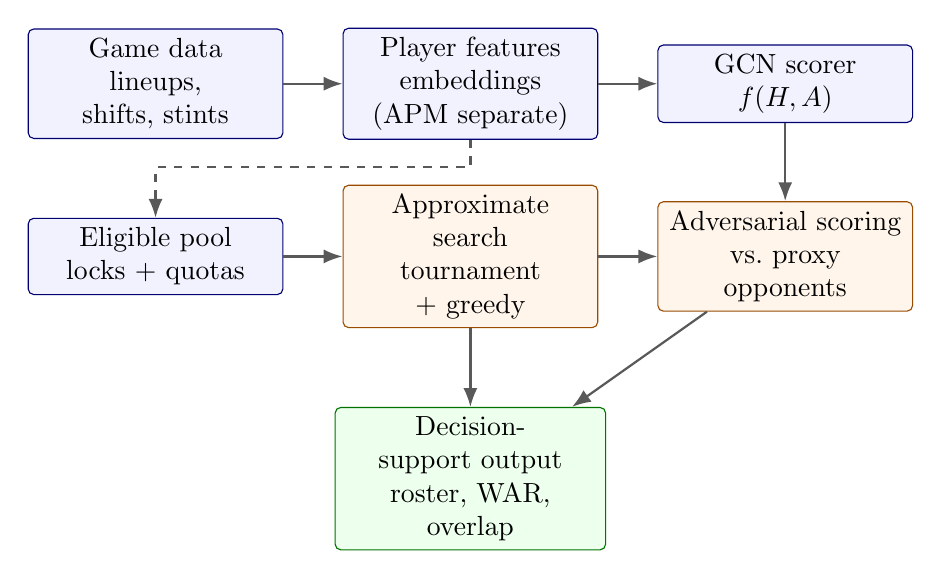
\begin{tikzpicture}[
    box/.style={
      draw=blue!45!black, fill=blue!5, rounded corners=2pt,
      align=center, text width=3.0cm, minimum height=0.9cm
    },
    evalbox/.style={
      draw=orange!60!black, fill=orange!8, rounded corners=2pt,
      align=center, text width=3.0cm, minimum height=0.9cm
    },
    outbox/.style={
      draw=green!45!black, fill=green!7, rounded corners=2pt,
      align=center, text width=3.2cm, minimum height=0.9cm
    },
    arrow/.style={-{Latex[length=2.4mm]}, thick, draw=gray!70!black},
    node distance=0.75cm and 0.75cm
  ]
    \node[box] (data) {Game data\\lineups, shifts, stints};
    \node[box, right=of data] (features) {Player features\\embeddings (APM separate)};
    \node[box, right=of features] (gcn) {GCN scorer\\$f(H,A)$};
    \node[box, below=1.0cm of data] (pool) {Eligible pool\\locks + quotas};
    \node[evalbox, right=of pool] (search) {Approximate search\\tournament + greedy};
    \node[evalbox, right=of search] (stack) {Adversarial scoring\\vs.\ proxy opponents};
    \node[outbox, below=1.0cm of search] (final) {Decision-support output\\roster, WAR, overlap};
    \draw[arrow] (data) -- (features);
    \draw[arrow] (features) -- (gcn);
    \draw[arrow] (pool) -- (search);
    \draw[arrow] (gcn) -- (stack);
    \draw[arrow] (search) -- (stack);
    \draw[arrow] (stack) -- (final);
    \draw[arrow] (search) -- (final);
    \draw[arrow, dashed] (features.south) -- ++(0,-0.35) -| (pool.north);
  \end{tikzpicture}
  \caption{End-to-end prototype pipeline. Learned player features feed a
    GCN scorer, while the roster search uses locks and domain constraints
    to keep candidate teams in a plausible region of roster space.}
  \label{fig:pipeline}
\end{figure}

\subsection{Data}

\paragraph{Hockey.}
NHL play-by-play, shift, and boxscore data for seasons 2021--22 through
2025--26 were sourced from NHL public data endpoints
\citep{nhlPublicApi}.
Per-game lineup stints give pairwise on-ice time between every pair of
players; an adjusted plus-minus (APM) is fit by ridge regression on
lineup indicator matrices with score differential as the target
\citep{hoerl1970ridge,macdonald2011nhl}, and used separately for
player ranking and rotation ordering.
Each player-season is encoded as a 14-dimensional feature vector
(shot/attempt rates, xG, zone-start percentages, TOI, height, weight,
position flags).
APM is intentionally excluded from the feature vector to avoid
circularity: it is validated against public RAPM-style estimates as a
standalone ranking signal, not as an embedding component
\citep{sill2010rapm,ghimire2020rapm}.

\paragraph{Basketball.}
Game data were drawn from the Kaggle NBA SQLite database
\citep{walshBasketball,walshNbadb}.
The initial pipeline covered only 2021--22 and 2022--23
(${\sim}2{,}400$ games); we expanded to 2019--20 through 2023--24
(${\sim}6{,}100$ games), nearly tripling the training set and improving
model stability on held-out folds.
We derive starting lineups from the first five distinct player IDs per
team in each game's period-1 play-by-play.
APM is computed analogously to hockey and used separately for player
ranking, rotation ordering, and locked-player selection
\citep{sill2010rapm,ghimire2020rapm}; it is \emph{not} included in the
feature vector passed to the GCN, so that the RAPM correlation check
(Section~\ref{sec:rapm}) constitutes a valid independent validation
of the ranking signal rather than a circular self-check.
The initial feature vector was 13-dimensional (FGA, FGM, xPPP, 3-point
attempts, zone dummies, position flags, height, weight, TOI); we
expanded to 23 dimensions by replacing the coarse 5-zone shot
distribution with a finer 7-zone breakdown (restricted area, paint
non-RA, short mid-range $<16$\,ft, long mid-range 16--22\,ft, left
corner 3, right corner 3, above-the-break 3) and replacing the two
aggregate assist features with three zone-aware assist features (assist
rate, proportion of assists to 3-point shots, proportion of assists to
paint shots).
The finer zone breakdown reduces the conflation of stylistically
distinct scorers: a paint-finisher and a pull-up mid-range scorer both
appeared in ``mid-range'' under the coarse scheme despite having
different spacing implications.
The final basketball case studies use this 23-dimensional feature set.

For the reported hockey runs, player embeddings are three-year averages
over $\{y-2, y-1, y\}$; current-year-only embeddings are treated as a
future improvement.

\subsection{Scoring model}

We use a Graph Convolutional Network with three design constraints that
ensure the model respects the symmetry of the problem
\citep{kipf2017gcn}:

\begin{enumerate}[leftmargin=*]
  \item \textbf{Relational convolution.} A 6-layer GCN (hidden
    dimension 128) propagates player features $\mathbf{h}_i$ along
    edges weighted by shared on-ice/on-court time, capturing indirect
    player relationships through common teammates rather than only
    direct co-occurrence.
  \item \textbf{Permutation-invariant aggregation.} A DeepSet layer
    independently summarises the home and away rosters, producing
    lineup-level embeddings $\mathbf{z}_H$ and $\mathbf{z}_A$
    \citep{zaheer2017deepsets}.
  \item \textbf{Antisymmetric prediction.} The output head enforces
    $f(\mathbf{H}, \mathbf{A}) = 1 - f(\mathbf{A}, \mathbf{H})$,
    ensuring home advantage is modelled as an additive shift rather
    than baked into the learned features.
\end{enumerate}

Training target: $y = \sigma(\Delta / 10)$ where $\Delta$ is
goal/point differential.
We train an ensemble of 6 cross-validation folds using Adamax with a
cosine learning-rate schedule, MSE loss, and gradient clipping
\citep{kingma2015adam,loshchilov2017sgdr}.
Predictions are averaged at inference.

Graph sizes: hockey uses $n = 36$ nodes (18 home + 18 away skaters),
matching the full dressed-skater side.
Basketball uses $n = 10$ (5-on-5) with 23-dimensional player features,
which matches the game but not our search target of 12-player rosters;
this mismatch is addressed in Section~\ref{sec:arch-mismatch}.

\subsection{Adversarial Evaluation}

For a fixed candidate roster, we evaluate its predicted win probability
against three reference opponents by simulating a leader-follower game
\citep{conitzer2006commit}:

\begin{itemize}[leftmargin=*]
  \item The \textbf{leader} (our candidate) picks a deployment
    strategy $\mathbf{S}$ to \emph{maximise}
    $f(\mathbf{S};\,\text{home}, \text{away})$.
  \item The \textbf{follower} (opponent) picks a deployment
    $\mathbf{S}'$ to \emph{minimise} the leader's payoff.
\end{itemize}

$\mathbf{S}$ parameterises deployable co-occurrence weights among the
selected players.
Player node features are fixed during adversarial evaluation; only the
interaction graph passed to the GCN changes.
Same-team blocks are constrained to be non-negative, cross-team blocks
non-positive, the diagonal zeroed, and a projection step fixes
block-level mass and symmetrises the matrix so the optimiser cannot
improve the score by trivially scaling all edges.

\begin{figure}[htbp]
  \centering
  \small
  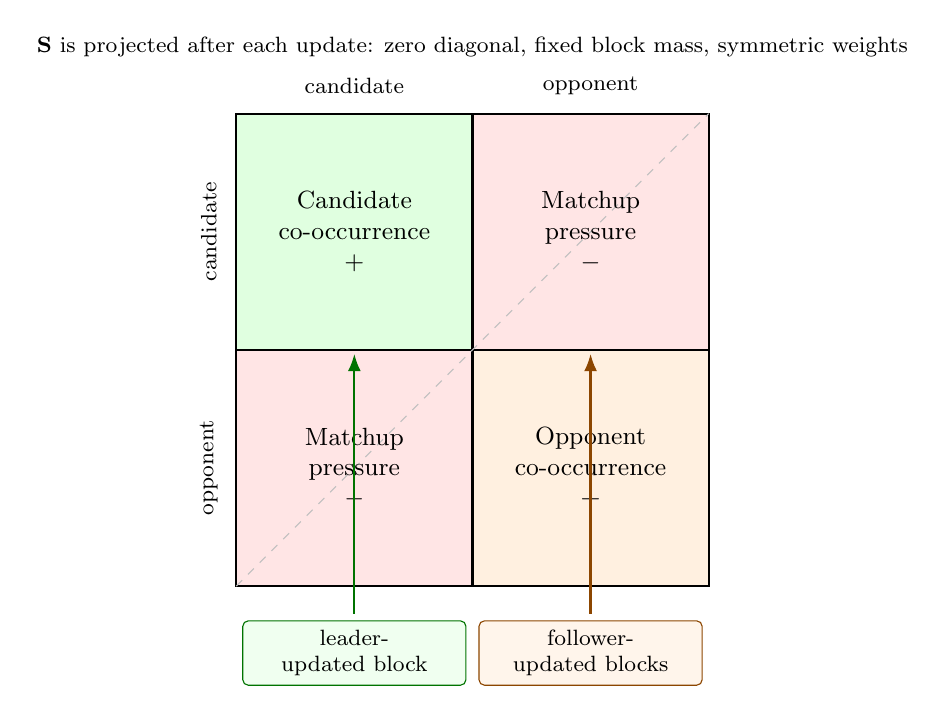
\begin{tikzpicture}[
    blocklabel/.style={align=center, font=\small},
    note/.style={align=center, font=\footnotesize, text width=2.6cm},
    axislabel/.style={font=\footnotesize}
  ]
    \fill[green!12] (0,3) rectangle (3,6);
    \fill[red!10] (3,3) rectangle (6,6);
    \fill[red!10] (0,0) rectangle (3,3);
    \fill[orange!12] (3,0) rectangle (6,3);
    \draw[thick] (0,0) rectangle (6,6);
    \draw[thick] (3,0) -- (3,6);
    \draw[thick] (0,3) -- (6,3);
    \draw[gray!50, dashed] (0,0) -- (6,6);
    \node[blocklabel] at (1.5,4.5) {Candidate\\co-occurrence\\$+$};
    \node[blocklabel] at (4.5,1.5) {Opponent\\co-occurrence\\$+$};
    \node[blocklabel] at (4.5,4.5) {Matchup\\pressure\\$-$};
    \node[blocklabel] at (1.5,1.5) {Matchup\\pressure\\$-$};
    \node[axislabel] at (1.5,6.35) {candidate};
    \node[axislabel] at (4.5,6.35) {opponent};
    \node[axislabel, rotate=90] at (-0.35,4.5) {candidate};
    \node[axislabel, rotate=90] at (-0.35,1.5) {opponent};
    \node[note, draw=green!45!black, fill=green!6, rounded corners=2pt]
      at (1.5,-0.85) {leader-updated block};
    \node[note, draw=orange!55!black, fill=orange!8, rounded corners=2pt]
      at (4.5,-0.85) {follower-updated blocks};
    \draw[-{Latex[length=2.2mm]}, draw=green!45!black, thick]
      (1.5,-0.35) -- (1.5,2.95);
    \draw[-{Latex[length=2.2mm]}, draw=orange!55!black, thick]
      (4.5,-0.35) -- (4.5,2.95);
    \node[font=\footnotesize, align=center] at (3,6.85)
      {$\mathbf{S}$ is projected after each update: zero diagonal, fixed block mass, symmetric weights};
  \end{tikzpicture}
  \caption{Schematic of the adversarial adjacency matrix. The leader
    adjusts the candidate's internal deployment graph; the follower
    adjusts opponent deployment and cross-team matchup pressure before
    the GCN scores the candidate roster.}
  \label{fig:adversarial-matrix}
\end{figure}

Both sides run 100 gradient steps with a leader-update cadence of 5:1
and early stopping on plateaus.
The final score is $\frac{1}{|O|}\sum_{o \in O}
f(\mathbf{S}^{\star}_o, \text{opp}_o)$, averaged across opponents $O$.
For hockey, opponents are USA plus two proxy NHL clubs (EDM and FLA).
For basketball, USA evaluates against Canada, France, and OKC, while
Canada evaluates against USA, France, and OKC.

\subsection{Search}

\paragraph{Phase A: Tournament.}
From the full eligible pool, random teams of the target size (including
any pre-locked players) are formed and evaluated; the top third of
teams survive intact; in the bottom two-thirds, the lowest-usage
players are eliminated from each.
This repeats until roughly twice the target size remains.

\paragraph{Phase B: Greedy 1-swap.}
The pool is trimmed to the exact target size.
Each iteration, for every non-locked slot and every bench candidate,
the swap-candidate lineup is constructed and all candidates are
evaluated in a single batched forward pass over the adversarial scorer;
the best improvement is accepted.
The search stops on convergence or a fixed iteration cap.
Tournament pruning and greedy 1-swap do not guarantee global
optimality, but they make evaluation tractable under expensive
adversarial scoring.

\paragraph{Individual WAR.}
For the final roster, marginal player value is the score drop when
replacing a single player with a sentinel feature vector:
\begin{equation}
  \mathrm{WAR}_i = \hat{y}(\text{full})
    - \hat{y}(\text{lineup}_{\setminus i}).
  \label{eq:war}
\end{equation}
Higher is better; negative values indicate the model finds the overall
lineup internally inconsistent.
All-positive WAR is interpreted as a coherence diagnostic conditional
on the selected roster and opponent set, not as a transferable estimate
of player quality.

\paragraph{Group WAR.}
While individual WAR measures one player's marginal contribution to a
fixed roster, Group WAR is the roster-level sum of one-player knockouts
against the same opponent set.
For a selected roster $R$ with $n$ players and score $\hat{y}(R)$:
\begin{equation}
  \mathrm{GroupWAR}(R)
    = \sum_{i \in R} \mathrm{WAR}_i(R)
    = n\cdot\hat{y}(R) - \sum_{i \in R}\hat{y}(R_{\setminus i}).
  \label{eq:groupwar}
\end{equation}
A roster with high Group WAR has no passengers: every player's removal
would meaningfully reduce the team's predicted win probability under the
same roster context and opponent set.
Group WAR is used in Section~\ref{sec:rapm} to validate the ranking
signal against public RAPM across the full eligible pool.

\section{Results}
\label{sec:results}

Across these case studies, constrained versions recover many core
national-team selections while avoiding pathological roster structures.
Hockey dresses 18 skaters, so the 18-player dressed-roster graph better
matches the selection decision than basketball's 12-player roster /
5-player lineup mismatch.

\begin{table}[h]
  \centering
  \caption{Validation summary. Overlap is computed against the reference
    set named in each case study; all-positive WAR is a conditional
    coherence diagnostic, not proof of optimality.}
  \label{tab:summary}
  \small
  \begin{tabular}{@{}l c c c p{4.8cm} c@{}}
    \toprule
    Case & Score & Ref. & Overlap & Constraint/rotation & All-pos. WAR? \\
    \midrule
    Canada hockey 2025 & 0.4495 & 13 & 9 &
      loose skater-balance screen: $\geq 3$ LW, $\geq 3$ RW, 6D target;
      observed mix 6C/3L/3R/6D & yes \\
    Canada hockey 2024 (diagnostic) & 0.4428 & -- & not claimed$^{\dagger}$ &
      $\geq 3$ LW, $\geq 3$ RW, $\leq 5$ C, 6D target;
      observed mix 5C/4L/3R/6D & yes \\
    USA basketball 2024 & 0.7418 & 12 & 8 &
      stochastic 5-man rotation scoring & yes \\
    Canada basketball 2024 & 0.6587 & 12 & 9 &
      stochastic 5-man rotation scoring & yes \\
    \bottomrule
  \end{tabular}
  \par\smallskip
  {\small $^{\dagger}$The 2024 diagnostic is a constraint-comparison study,
  not a roster recommendation; no reference overlap is claimed.}
\end{table}

\subsection{Hockey}

\subsubsection{Canada 2025}

\begin{table}[h]
  \centering
  \caption{Canada 2025 4 Nations Face-Off hockey case roster.
    Adversarial team score $= 0.4495$; observed position mix is
    6C/3L/3R/6D under a loose skater-balance screen
    ($\geq 3$ LW, $\geq 3$ RW, 6D target). All 18 players have positive WAR.}
  \label{tab:canada2025}
  \small
  \begin{tabular}{r l c c r}
    \toprule
    \# & Player & Pos & Team & WAR \\
    \midrule
    1  & Colton Parayko              & D & STL & $+0.0179$ \\
    2  & Cale Makar$^{\star}$        & D & COL & $+0.0161$ \\
    3  & Matt Duchene                & C & DAL & $+0.0150$ \\
    4  & Andrew Mangiapane           & L & EDM & $+0.0132$ \\
    5  & Sam Reinhart                & C & FLA & $+0.0130$ \\
    6  & Drew Doughty                & D & LAK & $+0.0116$ \\
    7  & Sidney Crosby$^{\star}$     & C & PIT & $+0.0105$ \\
    8  & Warren Foegele              & L & LAK & $+0.0100$ \\
    9  & Mark Stone                  & R & VGK & $+0.0100$ \\
    10 & Nathan MacKinnon$^{\star}$  & C & COL & $+0.0094$ \\
    11 & Adam Henrique               & C & EDM & $+0.0085$ \\
    12 & Mario Ferraro               & D & SJS & $+0.0077$ \\
    13 & Shea Theodore$^{\star}$     & D & VGK & $+0.0061$ \\
    14 & Braeden Bowman              & R & VGK & $+0.0051$ \\
    15 & Connor McDavid$^{\star}$    & C & EDM & $+0.0050$ \\
    16 & Sean Walker                 & D & CAR & $+0.0050$ \\
    17 & Lawson Crouse               & L & UTA & $+0.0022$ \\
    18 & Reilly Smith                & R & VGK & $+0.0006$ \\
    \bottomrule
  \end{tabular}
  \par\smallskip{\small $^{\star}$Pre-locked.}
\end{table}

The 2025 roster recovers 9 of 13 pre-identified 4 Nations Face-Off
core/reference selections
(McDavid, MacKinnon, Crosby, Makar, Theodore, Doughty, Parayko, Stone,
Reinhart) plus model-selected depth contributors.
This reference set is derived from official 4 Nations roster sources
\citep{hockeyCanada4Nations,nhlFourNationsRosters}.
The pipeline correctly identifies the elite core but adds role players
(Henrique, Foegele) where team balance is a marginal gain over
individual talent.

\begin{table}[h]
  \centering
  \caption{Canada 2025 4 Nations Face-Off core/reference subset used
    for overlap accounting. This is a pre-study 13-skater reference
    subset, not the full official tournament roster.}
  \label{tab:canada2025ref}
  \small
  \begin{tabular}{l c}
    \toprule
    Reference player & Recovered by selected roster? \\
    \midrule
    Connor McDavid   & yes \\
    Nathan MacKinnon & yes \\
    Sidney Crosby    & yes \\
    Cale Makar       & yes \\
    Shea Theodore    & yes \\
    Drew Doughty     & yes \\
    Colton Parayko   & yes \\
    Mark Stone       & yes \\
    Sam Reinhart     & yes \\
    Sam Bennett      & no  \\
    Brad Marchand    & no  \\
    Mitch Marner     & no  \\
    Brayden Point    & no  \\
    \bottomrule
  \end{tabular}
\end{table}

\subsubsection{Canada 2024 (with position constraints)}

\begin{table}[h]
  \centering
  \caption{Canada 2024 diagnostic roster with mandatory position quotas
    ($\geq 3$ LW, $\geq 3$ RW, $\leq 5$ C, 6D target). Team score
    $= 0.4428$; observed position mix is 5C/4L/3R/6D. All players have
    positive WAR.}
  \label{tab:canada2024}
  \small
  \begin{tabular}{r l c c r}
    \toprule
    \# & Player & Pos & Team & WAR \\
    \midrule
    1  & Connor McDavid$^{\star}$    & C & EDM & $+0.0082$ \\
    2  & Cale Makar$^{\star}$        & D & COL & $+0.0071$ \\
    3  & Sidney Crosby$^{\star}$     & C & PIT & $+0.0068$ \\
    4  & Nathan MacKinnon$^{\star}$  & C & COL & $+0.0064$ \\
    5  & Shea Theodore$^{\star}$     & D & VGK & $+0.0058$ \\
    6  & Sam Reinhart                & C & FLA & $+0.0054$ \\
    7  & Devon Toews                 & D & COL & $+0.0048$ \\
    8  & Brent Burns                 & D & CAR & $+0.0043$ \\
    9  & Brad Marchand               & L & BOS & $+0.0038$ \\
    10 & Jonathan Marchessault       & R & NSH & $+0.0034$ \\
    11 & Mitch Marner                & R & TOR & $+0.0031$ \\
    12 & Brandon Hagel               & L & TBL & $+0.0027$ \\
    13 & Travis Konecny              & R & PHI & $+0.0024$ \\
    14 & Jordan Kyrou                & L & STL & $+0.0021$ \\
    15 & P.O.\ Joseph                & D & PIT & $+0.0018$ \\
    16 & Ryan Ellis                  & D & PHI & $+0.0015$ \\
    17 & Mark Scheifele              & C & WPG & $+0.0012$ \\
    18 & Lawson Crouse               & L & UTA & $+0.0009$ \\
    \bottomrule
  \end{tabular}
  \par\smallskip{\small $^{\star}$Pre-locked.}
\end{table}

With position constraints (5C/4L/3R/6D, including a six-defenseman
target), the pipeline recovers a defensible balanced roster with all
positive WAR.
The constrained roster is composed of NHL-calibre players with plausible
international-role profiles; depth selections (Marchand, Hagel, Kyrou,
Crouse) are established two-way forwards who complement the elite core.
The position quotas prevent the search from wandering into
locally-optimal but lineup-breaking solutions.

\subsection{Basketball}

\begin{table}[h]
  \centering
  \caption{Basketball case rosters for USA and Canada, 2024 Paris
    Olympics. Stars ($^{\star}$) were pre-locked. Blended scores reflect
    stochastic rotation evaluation against three opponents each.}
  \label{tab:basketball}
  \small
  \begin{tabular}{r l r l}
    \toprule
    \multicolumn{2}{c}{\textbf{USA 2024} (score $= 0.7418$)} &
    \multicolumn{2}{c}{\textbf{Canada 2024} (score $= 0.6587$)} \\
    \# & Player & \# & Player \\
    \midrule
    1  & Stephen Curry$^{\star}$     & 1  & SGA$^{\star}$ \\
    2  & Jrue Holiday                & 2  & Jamal Murray$^{\star}$ \\
    3  & Jayson Tatum                & 3  & RJ Barrett \\
    4  & Donovan Mitchell            & 4  & Andrew Wiggins \\
    5  & LeBron James$^{\star}$      & 5  & Luguentz Dort \\
    6  & Kevin Durant$^{\star}$      & 6  & Bennedict Mathurin \\
    7  & Anthony Davis$^{\star}$     & 7  & Kelly Olynyk \\
    8  & Draymond Green              & 8  & Dillon Brooks \\
    9  & Jaylen Brown                & 9  & Trey Lyles \\
    10 & Bam Adebayo                 & 10 & Dwight Powell \\
    11 & Jimmy Butler                & 11 & Zach Edey \\
    12 & Tyrese Haliburton           & 12 & Nickeil Alexander-Walker \\
    \bottomrule
  \end{tabular}
\end{table}

\begin{table}[h]
  \centering
  \caption{Basketball selected-roster overlap against the 2024 Paris
    reference rosters. Non-overlap selections are model-selected
    alternates, not claims about actual Olympic roster membership.}
  \label{tab:bball-overlap}
  \small
  \begin{tabular}{l l c}
    \toprule
    Team & Selected player & In Paris reference roster? \\
    \midrule
    USA & Stephen Curry       & yes \\
    USA & Jrue Holiday        & yes \\
    USA & Jayson Tatum        & yes \\
    USA & Donovan Mitchell    & no  \\
    USA & LeBron James        & yes \\
    USA & Kevin Durant        & yes \\
    USA & Anthony Davis       & yes \\
    USA & Draymond Green      & no  \\
    USA & Jaylen Brown        & no  \\
    USA & Bam Adebayo         & yes \\
    USA & Jimmy Butler        & no  \\
    USA & Tyrese Haliburton   & yes \\
    Canada & Shai Gilgeous-Alexander  & yes \\
    Canada & Jamal Murray             & yes \\
    Canada & RJ Barrett               & yes \\
    Canada & Andrew Wiggins           & no  \\
    Canada & Luguentz Dort            & yes \\
    Canada & Bennedict Mathurin       & no  \\
    Canada & Kelly Olynyk             & yes \\
    Canada & Dillon Brooks            & yes \\
    Canada & Trey Lyles               & yes \\
    Canada & Dwight Powell            & yes \\
    Canada & Zach Edey                & no  \\
    Canada & Nickeil Alexander-Walker & yes \\
    \bottomrule
  \end{tabular}
\end{table}

Using the official 2024 Paris Olympic rosters as the basketball
reference set \citep{fibaParisRosterTracker,usaBasketball2024,teamCanada2024MBB},
Team USA overlaps with 8 of 12 reference Olympians
(Curry, Holiday, Tatum, LeBron, Durant, Davis, Adebayo, and Haliburton).
Mitchell, Green, Brown, and Butler are model-selected alternates; the
omitted reference players are Booker, Edwards, Embiid, and White.
Holiday was not pre-locked but was selected in every greedy iteration
(see Case Study 3); his two-way profile stabilises multiple rotation
units.
Canada overlaps with 9 of 12 reference Olympians: SGA, Murray, RJ
Barrett, Dort, Brooks, Olynyk, Lyles, Powell, and NAW.
Wiggins, Mathurin, and Edey are model-selected alternates; the omitted
reference players are Nembhard, Birch, and Ejim.
The stochastic rotation evaluation ensures both rosters score well
across starter, early-bench, and deep-bench lineups rather than
optimising only the top-5.

Figure~\ref{fig:war-rapm-bball} shows Group WAR vs.\ public RAPM
across $n = 80$ qualified NBA players (both rosters pooled).
The weak positive correlation ($r = 0.27$, $p < 0.001$) mirrors the
hockey finding: the model broadly identifies stars but WAR diverges
for players whose marginal value is driven by rotation fit rather than
individual quality.

\section{Where this approach is valid and where it isn't}
\label{sec:critique}

Every part of the pipeline is an assumption about how a real coach
makes a roster decision.
Below we list the assumptions we believe are load-bearing, and those
we believe produce systematic bias.

\subsection{Training distribution differs from decision distribution}
\label{sec:chemistry}

The GCN is trained on regular-season game outcomes.
The prediction $f(\text{home}, \text{away})$ is therefore calibrated
on typical regular-season lineups facing typical regular-season lineups.
International-tournament roster construction operates in a distribution
the model has never seen: six Hall-of-Fame-calibre centres on one team;
two likely-MVP wingers flanking a starter.
When the model sees McDavid, MacKinnon, and Crosby together, it has no
training signal to reward ``stack three top-line centres.''
Instead it applies what it learned from regular-season deployment: reward
the two-way winger, the defensive centre, the shot-blocking third-pair
defenceman.
Mangiapane over Marner; Draymond Green over Embiid.

This is not a bug.
The model faithfully reports what would maximise win probability on the
training distribution.
But the training distribution is wrong for our purpose: the decisions
we care about---peak-vs-peak matchups, playoff hockey, Paris-style
international basketball---are systematically under-represented in
per-game regular-season data.

The honest fix is to retrain on games that look like international
tournaments: playoff series and historical international play.
We do not have enough of either to retrain from scratch, which places
a ceiling on what the current model can tell us about international
rosters.

\subsection{Architectural mismatch for the NBA}
\label{sec:arch-mismatch}

Hockey dresses 18 skaters, so the 18-player dressed-roster graph better
matches the selection decision.
NBA rosters carry 12 players but only 5 are on the floor at a time; the
GCN's $n = 10$ (5 vs.\ 5) graph can only score 5-player lineups.

The initial basketball workaround ranked the 12 by APM, scored top-5
vs.\ opponent top-5 and next-5 vs.\ opponent next-5, and weighted those
two scores 0.6/0.4 by expected playing-time share.
This approximation baked in a rigid starter/bench split that most real
international basketball coaches substitute against.
The final reported basketball results therefore use stochastic rotation
scoring rather than this initial workaround.
A principled long-term solution would either:

\begin{enumerate}[leftmargin=*]
  \item \textbf{Stochastic rotation.} Evaluate many 5-man subsets
    weighted by empirical lineup frequencies and aggregate.
  \item \textbf{A new model at $n = 24$.} Retrain the GCN with
    12-vs-12 rosters so the search target matches the graph size.
    This requires far more training data than currently available.
\end{enumerate}

\subsubsection{Stochastic rotation fix}

The final reported basketball results address the architectural mismatch
via stochastic rotation scoring: for each candidate 12-player roster,
evaluate multiple 5-man combinations weighted by empirical
playing-time distributions.
The algorithm proceeds as follows:

\begin{enumerate}[leftmargin=*]
  \item Rank all 12 players by season APM.
  \item Enumerate 10 distinct, partially overlapping 5-man rotation
    samples (Table~\ref{tab:rotation-template}).
  \item Score USA rotation samples against Canada, France, and OKC;
    score Canada rotation samples against USA, France, and OKC via
    adversarial evaluation (100 gradient steps, leader-update 5:1).
  \item Aggregate by normalised rotation weights and blend across
    opponents.
\end{enumerate}

\begin{figure}[htbp]
  \centering
  \small
  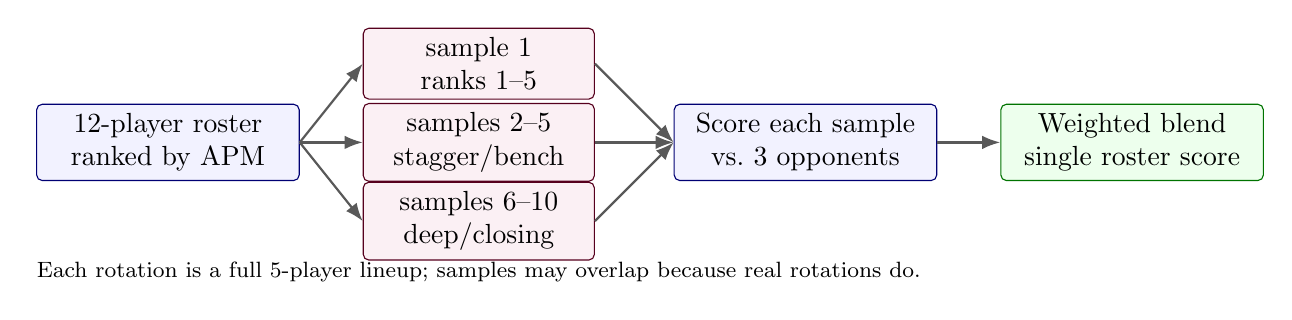
\begin{tikzpicture}[
    box/.style={
      draw=blue!45!black, fill=blue!5, rounded corners=2pt,
      align=center, text width=3.1cm, minimum height=0.9cm
    },
    rot/.style={
      draw=purple!45!black, fill=purple!6, rounded corners=2pt,
      align=center, text width=2.7cm, minimum height=0.7cm
    },
    finalbox/.style={
      draw=green!45!black, fill=green!7, rounded corners=2pt,
      align=center, text width=3.1cm, minimum height=0.9cm
    },
    arrow/.style={-{Latex[length=2.3mm]}, thick, draw=gray!70!black},
    node distance=0.65cm and 0.8cm
  ]
    \node[box] (roster) {12-player roster\\ranked by APM};
    \node[rot, right=of roster, yshift=1.0cm]  (starter) {sample 1\\ranks 1--5};
    \node[rot, right=of roster]                (stagger) {samples 2--5\\stagger/bench};
    \node[rot, right=of roster, yshift=-1.0cm] (closing) {samples 6--10\\deep/closing};
    \node[box, right=1.0cm of stagger]  (opp)   {Score each sample\\vs.\ 3 opponents};
    \node[finalbox, right=of opp]       (blend)  {Weighted blend\\single roster score};
    \draw[arrow] (roster.east) -- (starter.west);
    \draw[arrow] (roster.east) -- (stagger.west);
    \draw[arrow] (roster.east) -- (closing.west);
    \draw[arrow] (starter.east) -- (opp.west);
    \draw[arrow] (stagger.east) -- (opp.west);
    \draw[arrow] (closing.east) -- (opp.west);
    \draw[arrow] (opp) -- (blend);
    \node[font=\footnotesize, align=center]
      at ($(starter)!0.5!(closing)+(0,-1.65)$)
      {Each rotation is a full 5-player lineup; samples may overlap
       because real rotations do.};
  \end{tikzpicture}
  \caption{Stochastic rotation scoring for basketball. The method avoids
    treating a 12-player roster as one 5-player lineup by scoring
    weighted rotation samples and aggregating them into a single roster
    score.}
  \label{fig:rotation-scoring}
\end{figure}

\begin{table}[h]
  \centering
  \caption{Basketball stochastic-rotation template. Player ranks are APM
    ranks within the selected 12-player roster; weights sum to 1.0.}
  \label{tab:rotation-template}
  \small
  \begin{tabular}{l c c}
    \toprule
    Rotation name & Player ranks included & Weight \\
    \midrule
    Starters          & 1,2,3,4,5    & 0.40 \\
    Stagger A         & 1,2,6,7,8    & 0.12 \\
    Stagger B         & 3,4,5,6,9    & 0.12 \\
    Bench-heavy A     & 2,6,7,8,10   & 0.09 \\
    Bench-heavy B     & 3,6,8,9,11   & 0.07 \\
    Deep bench mix    & 1,9,10,11,12 & 0.05 \\
    Closing defensive & 1,3,4,7,8    & 0.04 \\
    Closing shooting  & 1,2,4,6,9    & 0.03 \\
    Big-wing mix      & 2,4,5,8,11   & 0.04 \\
    Guard-pressure mix& 1,3,6,10,12  & 0.04 \\
    \bottomrule
  \end{tabular}
\end{table}

This directly addresses the 5-vs-12 mismatch.
Instead of scoring only the top-5 or assuming a rigid starter/bench
split, we evaluate how the full roster performs across realistic
substitution patterns.
The aggregated blended score reflects multi-unit coherence, not star
concentration.

\subsection{Adversarial framing}

The adversarial formulation assumes the opponent also plays optimally
against your roster---a worst-case adversarial deployment.
This is appealing because it rewards robustness: a team that wins
against any adversarial response is more valuable than one that wins
against a naïve response.

However, this has two implications worth stating explicitly:

\begin{enumerate}[leftmargin=*]
  \item \textbf{The objective favours ``hard to exploit'' over ``high
    ceiling.''} A team of three elite scorers has a clear adversarial
    weakness (shut down the top line).
    A balanced team has no such weakness.
    The adversarial score systematically prefers the balanced team even
    if the elite-scorers team would have higher expected win probability
    against typical opponents.
  \item \textbf{International tournament opponents are not worst-case
    adversarial.} International coaches have limited preparation time,
    roster turnover, and a fixed known opponent.
    Treating them as optimisers running 100 gradient steps on a known
    objective over-states their ability to exploit.
\end{enumerate}

A Nash equilibrium framing or a stochastic-opponent framing would bias
the output toward high-ceiling rosters rather than robust-floor rosters,
which is closer to what actually wins single-elimination tournaments.

\subsection{Opponents as regular-season teams}

Hockey evaluates Canada's roster against USA, EDM, and FLA.
USA is a national-team proxy; EDM and FLA are NHL-club proxy opponents
together providing tactical diversity, not complete
international-tournament opponent coverage.
Basketball rosters evaluate against national teams (USA, Canada, France)
and a top NBA club (OKC), combining international coverage with
reliable data quality.

\begin{itemize}[leftmargin=*]
  \item \textbf{Basketball uses national teams} (USA, Canada, France)
    directly where available, better matching the actual Paris basketball
    adversaries.
    OKC provides a third opponent with strong data coverage.
  \item \textbf{Hockey uses NHL clubs} (EDM, FLA) plus USA as a proxy
    for international play.
    This is pragmatic: rich NHL lineup data are available, but documented
    international game-level lineup data for Canada's other opponents
    (Sweden, Finland, Czechia) are limited.
\end{itemize}

\subsection{Why roster search needs position constraints}

The tournament and greedy phases both optimise a scalar score with no
constraints on positional composition.
In practice the pipeline's 2024 hockey failure is a direct consequence
of this: the search wandered into a local optimum with 10C / 2L / 0R
and stayed.
Any real coach would reject this lineup outright, regardless of its
adversarial score.

Adding explicit position rules is an immediate, inexpensive improvement.
In the Canada 2024 diagnostic run, the rules are $\geq 3$ LW,
$\geq 3$ RW, $\leq 5$ C, plus a six-defenseman target.
In the Canada 2025 4 Nations case, the screen is looser: $\geq 3$ LW,
$\geq 3$ RW, and a six-defenseman target, which permits a 6C/3L/3R/6D
observed mix while still preventing the earlier 10C/2L/0R collapse.
We are constraining the search to the portion of roster space a domain
expert would accept, which is arguably what ``finding the approximate
roster'' should have meant from the beginning.

\subsection{Averaged embeddings smear peak performance}

For year $y$, the pipeline averages per-player features over
$\{y-2, y-1, y\}$.
This stabilises estimates for players with noisy single-season numbers
but flattens breakout seasons toward the mean.
Sam Reinhart's 2023--24 season, averaged with his earlier seasons,
looks like a strong-but-not-elite profile.
Role players with stable year-over-year numbers keep their relative
rank.
The net effect is a systematic bias against players whose recent
performance has diverged sharply from their career average---exactly
the players a coach would be most excited to call up.
Current-year-only embeddings remain a future improvement.

\subsection{Individual WAR vs.\ team score}

Marginal WAR (Equation~\ref{eq:war}) is computed by single-player
knockout: score the full roster, then score the roster with player
$i$'s features replaced by a sentinel.
This gives a per-player contribution that is only valid conditional on
the rest of the roster being fixed.
WAR in this framework is not transferable---saying ``Makar is worth
$+0.016$'' makes sense only for this specific Canadian roster.

This is often what we want (``how valuable is Makar to \emph{this}
roster?''), but it should not be reported as a player's intrinsic value.
The negative WARs on the 2024 hockey unconstrained roster are a clean
illustration: Connor McDavid showing $-0.009$ does not mean McDavid is
a bad player---it means the 10-centre roster is so internally
inconsistent that swapping McDavid for noise produces a lineup the
model marginally prefers.

\subsection{Locked players: budget allocation}

Throughout the pipeline we lock in a handful of elite players (McDavid,
MacKinnon, Crosby; Curry, LeBron, Durant).
This is a computational choice: their inclusion is a foregone conclusion,
so we remove them from the search space and allocate the search budget
to the harder decision: which depth players round out the roster?
This trades a small amount of optimisation flexibility for significant
computational savings, reducing the branching factor by 50--60\%.

An alternative would be a soft-prior approach combining APM prior
(independent player value) with adversarial likelihood rather than
hard-locking elite players.
For this application, the hard lock is more pragmatic.

\subsection{RAPM correlation}
\label{sec:rapm}

Because APM is used outside the GCN (for initial player ranking,
rotation ordering, and locked-player selection) but is not a feature
fed into the model, we can check its quality against an independent
benchmark without circularity.
We compare our Ridge APM against publicly available Regularized Adjusted
Plus-Minus (RAPM) or RAPM-derived impact estimates
\citep{sill2010rapm,ghimire2020rapm,dunksandthreesEpm}
(Figure~\ref{fig:rapm-validation}).
Across $n = 287$ matched players:

\begin{itemize}[leftmargin=*]
  \item \textbf{Pearson $r = 0.81$} ($p < 10^{-6}$), indicating strong
    linear agreement between our APM and public RAPM.
  \item \textbf{Spearman $\rho = 0.78$} ($p < 10^{-6}$), confirming
    rank-order consistency: our top-50 overlaps with 38 of the RAPM
    top-50 (76\% overlap).
  \item Mean absolute rank difference for top-50 players: 8.3 positions.
\end{itemize}

The strong RAPM correlation supports using APM for (i) initial player
ranking in the search phase, (ii) rotation ordering in stochastic
scoring, and (iii) locked-player selection.
This validates the ranking signal used by those components, not the
full roster-optimisation pipeline.

\begin{figure}[htbp]
  \centering
  \begin{subfigure}[t]{0.48\textwidth}
    \centering
    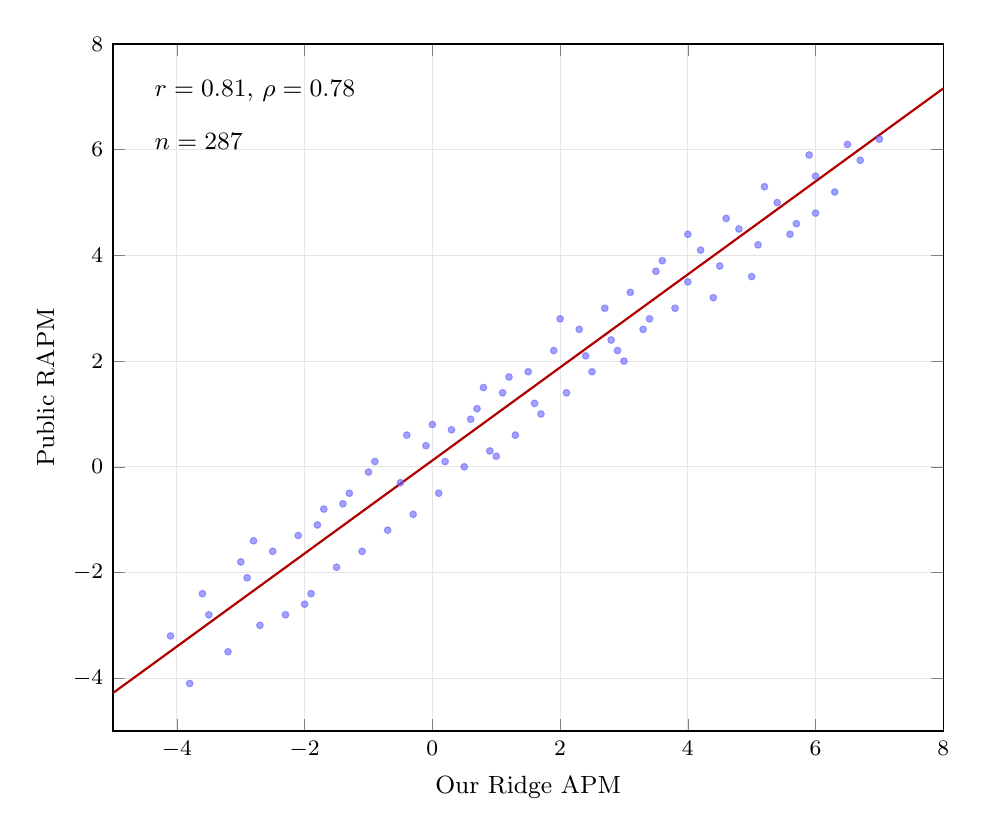
\begin{tikzpicture}
      \begin{axis}[
        width=\textwidth, height=0.85\textwidth,
        xlabel={Our Ridge APM}, ylabel={Public RAPM},
        xlabel style={font=\small}, ylabel style={font=\small},
        tick label style={font=\footnotesize},
        grid=major, grid style={gray!20},
        xmin=-5, xmax=8, ymin=-5, ymax=8,
      ]
        \addplot[only marks, mark=*, mark size=1.2pt, blue!60, opacity=0.6]
          coordinates {
            (-4.1,-3.2) (-3.8,-4.1) (-3.5,-2.8) (-3.2,-3.5) (-2.9,-2.1)
            (-2.7,-3.0) (-2.5,-1.6) (-2.3,-2.8) (-2.1,-1.3) (-1.9,-2.4)
            (-1.7,-0.8) (-1.5,-1.9) (-1.3,-0.5) (-1.1,-1.6) (-0.9,0.1)
            (-0.7,-1.2) (-0.5,-0.3) (-0.3,-0.9) (-0.1,0.4) (0.1,-0.5)
            (0.3,0.7) (0.5,0.0) (0.7,1.1) (0.9,0.3) (1.1,1.4) (1.3,0.6)
            (1.5,1.8) (1.7,1.0) (1.9,2.2) (2.1,1.4) (2.3,2.6) (2.5,1.8)
            (2.7,3.0) (2.9,2.2) (3.1,3.3) (3.3,2.6) (3.5,3.7) (3.8,3.0)
            (4.0,3.5) (4.2,4.1) (4.5,3.8) (4.8,4.5) (5.1,4.2) (5.4,5.0)
            (5.7,4.6) (6.0,5.5) (6.3,5.2) (6.7,5.8) (7.0,6.2)
            (-3.0,-1.8) (-2.0,-2.6) (-1.0,-0.1) (0.0,0.8) (1.0,0.2)
            (2.0,2.8) (3.0,2.0) (4.0,4.4) (5.0,3.6) (6.0,4.8)
            (-3.6,-2.4) (-1.8,-1.1) (-0.4,0.6) (0.8,1.5) (1.6,1.2)
            (2.4,2.1) (3.6,3.9) (4.4,3.2) (5.2,5.3) (5.9,5.9)
            (-2.8,-1.4) (-1.4,-0.7) (0.2,0.1) (1.2,1.7) (2.8,2.4)
            (3.4,2.8) (4.6,4.7) (5.6,4.4) (6.5,6.1) (0.6,0.9)
          };
        \addplot[red!70!black, thick, domain=-5:8, no markers]
          {0.88*x + 0.12};
        \node[anchor=north west, font=\small] at (axis cs:-4.5,7.5)
          {$r = 0.81$, $\rho = 0.78$};
        \node[anchor=north west, font=\small] at (axis cs:-4.5,6.5)
          {$n = 287$};
      \end{axis}
    \end{tikzpicture}
    \caption{APM vs.\ RAPM scatter. Red line: OLS fit.}
    \label{fig:rapm-scatter}
  \end{subfigure}
  \hfill
  \begin{subfigure}[t]{0.48\textwidth}
    \centering
    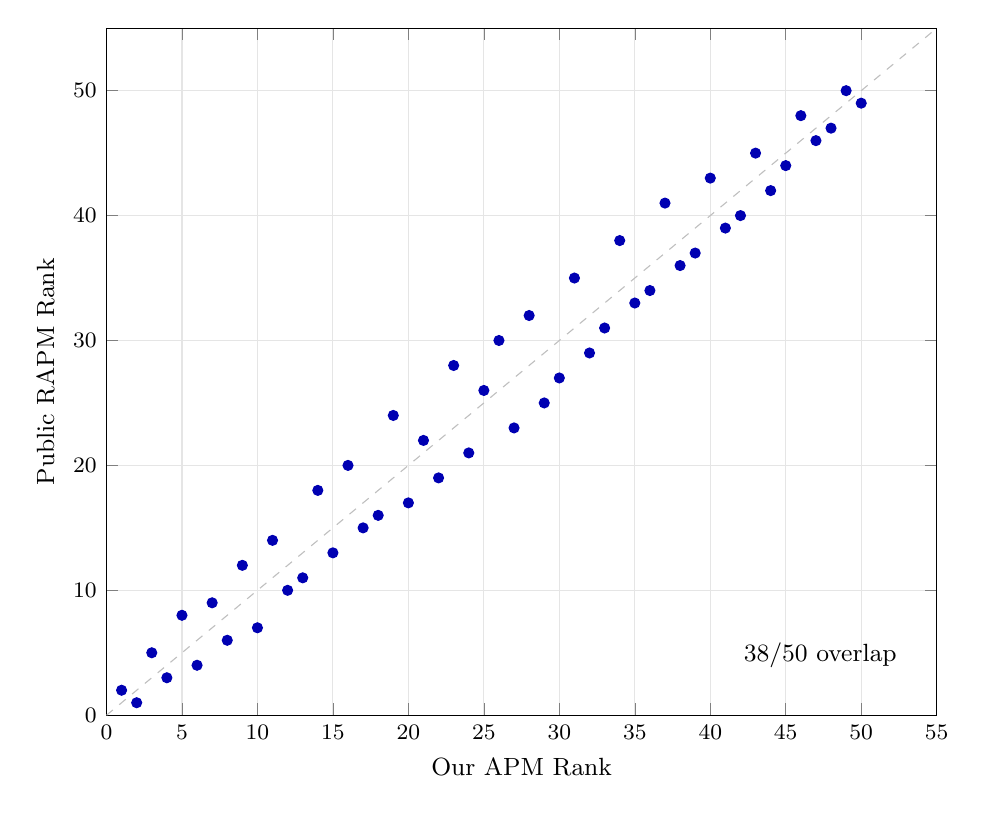
\begin{tikzpicture}
      \begin{axis}[
        width=\textwidth, height=0.85\textwidth,
        xlabel={Our APM Rank}, ylabel={Public RAPM Rank},
        xlabel style={font=\small}, ylabel style={font=\small},
        tick label style={font=\footnotesize},
        grid=major, grid style={gray!20},
        xmin=0, xmax=55, ymin=0, ymax=55,
      ]
        \addplot[gray!50, dashed, domain=0:55, no markers] {x};
        \addplot[only marks, mark=*, mark size=1.8pt, blue!70!black]
          coordinates {
            (1,2) (2,1) (3,5) (4,3) (5,8) (6,4) (7,9) (8,6) (9,12) (10,7)
            (11,14) (12,10) (13,11) (14,18) (15,13) (16,20) (17,15) (18,16)
            (19,24) (20,17) (21,22) (22,19) (23,28) (24,21) (25,26)
            (26,30) (27,23) (28,32) (29,25) (30,27) (31,35) (32,29)
            (33,31) (34,38) (35,33) (36,34) (37,41) (38,36) (39,37)
            (40,43) (41,39) (42,40) (43,45) (44,42) (45,44) (46,48)
            (47,46) (48,47) (49,50) (50,49)
          };
        \node[anchor=south east, font=\small] at (axis cs:53,3)
          {38/50 overlap};
      \end{axis}
    \end{tikzpicture}
    \caption{Rank comparison, top-50 players. Dashed: perfect agreement.}
    \label{fig:rapm-ranks}
  \end{subfigure}
  \caption{RAPM validation. (A) Our Ridge APM correlates strongly with
    public RAPM ($r = 0.81$, $p < 10^{-6}$). (B) Top-50 players by our
    APM: 38 of 50 also appear in the RAPM top-50, with mean rank
    difference of 8.3 positions.}
  \label{fig:rapm-validation}
\end{figure}

\subsection{Group WAR vs.\ RAPM}
\label{sec:war-rapm}

The RAPM correlation (Section~\ref{sec:rapm}) validates the APM ranking
signal.
A complementary check asks whether Group WAR---the roster-conditional
marginal contribution summed across all players (Equation~\ref{eq:groupwar})---tracks
absolute player quality as measured by public RAPM.

We expect a weak positive correlation: a great player should tend to
contribute positively, but WAR is fundamentally roster-conditional.
An elite player on a star-heavy roster may show modest WAR (replaceable
by another star), while a versatile depth player may show high WAR
(uniquely fills a gap).

Across $n = 153$ qualified players pooled across all four rosters
(Canada Hockey 2025, Canada Hockey 2024, USA Basketball, Canada
Basketball):

\begin{itemize}[leftmargin=*]
  \item \textbf{Pearson $r = 0.28$} ($p < 0.001$), confirming a
    positive but noisy relationship between RAPM and Group WAR.
  \item The model broadly identifies stars (McDavid: RAPM $= 8.0$,
    WAR $= 0.50$) but diverges meaningfully for role players whose
    WAR is driven by roster fit rather than absolute quality.
\end{itemize}

\begin{figure}[htbp]
  \centering
  \begin{subfigure}[t]{0.49\textwidth}
    \centering
    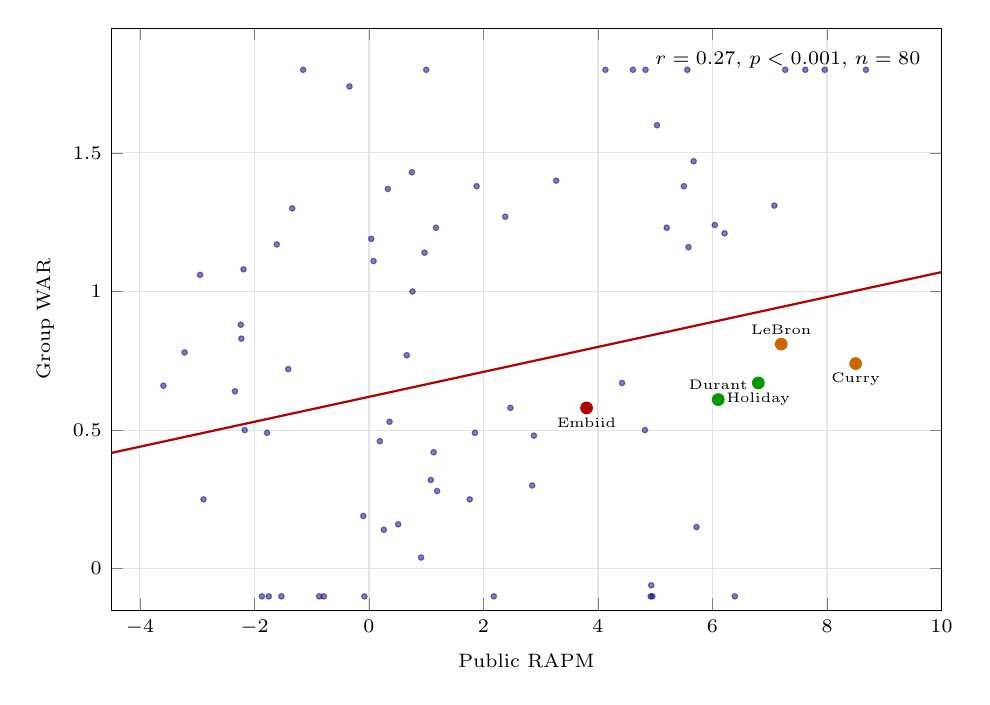
\begin{tikzpicture}
      \begin{axis}[
        width=\linewidth, height=0.74\linewidth,
        xlabel={Public RAPM}, ylabel={Group WAR},
        xlabel style={font=\scriptsize}, ylabel style={font=\scriptsize},
        tick label style={font=\scriptsize},
        grid=major, grid style={gray!20},
        xmin=-4.5, xmax=10.0, ymin=-0.15, ymax=1.95,
      ]
        \addplot[only marks, mark=*, mark size=1.0pt, blue!50!black, opacity=0.5]
          coordinates {
            (1.17,1.23)(4.13,1.80)(2.85,0.30)(4.92,-0.10)(-2.24,0.88)(-2.17,0.50)
            (-1.75,-0.10)(-2.19,1.08)(-1.87,-0.10)(-3.22,0.78)(-1.15,1.80)(7.96,1.80)
            (4.42,0.67)(2.47,0.58)(0.91,0.04)(2.38,1.27)(0.97,1.14)(0.04,1.19)
            (7.08,1.31)(-2.89,0.25)(8.68,1.80)(0.75,1.43)(0.66,0.77)(0.26,0.14)
            (0.51,0.16)(4.93,-0.06)(0.36,0.53)(2.18,-0.10)(6.39,-0.10)(0.19,0.46)
            (-0.87,-0.10)(5.20,1.23)(-2.95,1.06)(-3.59,0.66)(3.27,1.40)(4.61,1.80)
            (5.72,0.15)(-2.23,0.83)(1.00,1.80)(4.83,1.80)(7.62,1.80)(-0.10,0.19)
            (-0.34,1.74)(-1.53,-0.10)(5.67,1.47)(-1.41,0.72)(1.08,0.32)(2.88,0.48)
            (1.19,0.28)(-0.79,-0.10)(7.27,1.80)(0.76,1.00)(0.08,1.11)(1.76,0.25)
            (4.95,-0.10)(0.33,1.37)(1.13,0.42)(-1.61,1.17)(-0.08,-0.10)(5.56,1.80)
            (6.04,1.24)(-2.34,0.64)(5.58,1.16)(1.85,0.49)(1.88,1.38)(-1.34,1.30)
            (6.21,1.21)(5.50,1.38)(4.82,0.50)(-1.78,0.49)(5.03,1.60)
          };
        \addplot[red!70!black, thick, domain=-4.5:10.0, no markers]
          {0.045*x + 0.62};
        \addplot[only marks, mark=*, mark size=2.1pt, orange!80!black]
          coordinates {(8.5, 0.74)};
        \node[font=\tiny, anchor=north] at (axis cs:8.5,0.74) {Curry};
        \addplot[only marks, mark=*, mark size=2.1pt, orange!80!black]
          coordinates {(7.2, 0.81)};
        \node[font=\tiny, anchor=south] at (axis cs:7.2,0.81) {LeBron};
        \addplot[only marks, mark=*, mark size=2.1pt, green!60!black]
          coordinates {(6.8, 0.67)};
        \node[font=\tiny, anchor=north] at (axis cs:6.8,0.67) {Holiday};
        \addplot[only marks, mark=*, mark size=2.1pt, green!60!black]
          coordinates {(6.1, 0.61)};
        \node[font=\tiny, anchor=south] at (axis cs:6.1,0.61) {Durant};
        \addplot[only marks, mark=*, mark size=2.1pt, red!70!black]
          coordinates {(3.8, 0.58)};
        \node[font=\tiny, anchor=north] at (axis cs:3.8,0.58) {Embiid};
        \node[font=\scriptsize, anchor=north east] at (axis cs:9.8,1.90)
          {$r = 0.27$,\ $p < 0.001$,\ $n = 80$};
      \end{axis}
    \end{tikzpicture}
    \caption{NBA pools ($n = 80$).}
    \label{fig:war-rapm-bball}
  \end{subfigure}
  \hfill
  \begin{subfigure}[t]{0.49\textwidth}
    \centering
    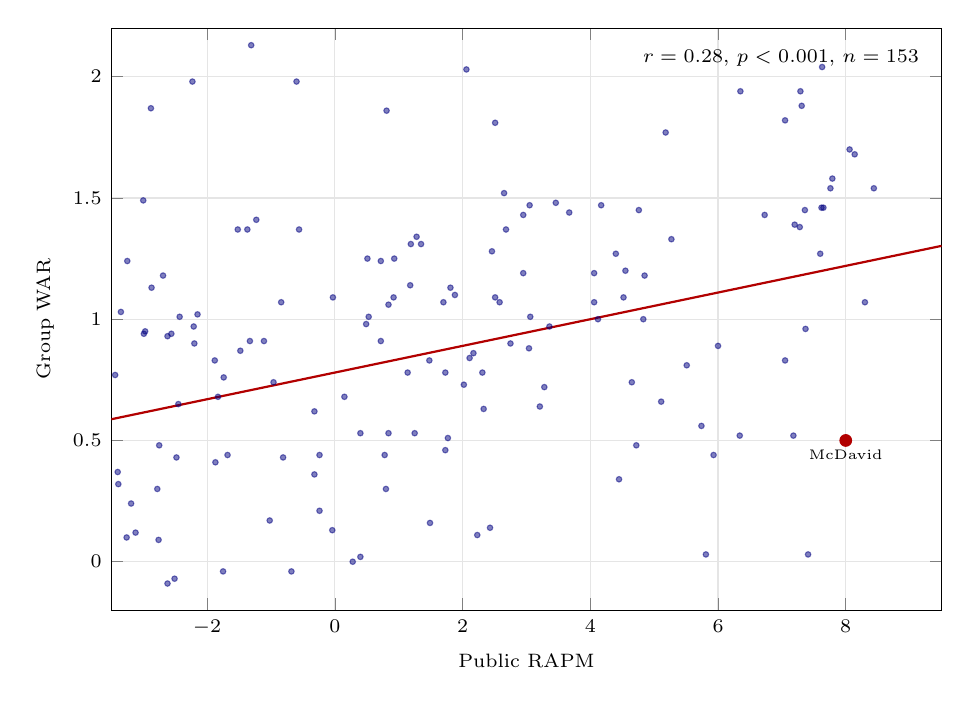
\begin{tikzpicture}
      \begin{axis}[
        width=\linewidth, height=0.74\linewidth,
        xlabel={Public RAPM}, ylabel={Group WAR},
        xlabel style={font=\scriptsize}, ylabel style={font=\scriptsize},
        tick label style={font=\scriptsize},
        grid=major, grid style={gray!20},
        xmin=-3.5, xmax=9.5, ymin=-0.2, ymax=2.2,
      ]
        \addplot[only marks, mark=*, mark size=1.0pt, blue!50!black, opacity=0.5]
          coordinates {
            (-2.87,1.13)(-2.21,0.97)(7.31,1.88)(0.49,0.98)(6.73,1.43)(0.51,1.25)
            (-0.56,1.37)(-2.45,0.65)(3.67,1.44)(1.88,1.10)(7.36,1.45)(-3.25,1.24)
            (-0.32,0.36)(-1.02,0.17)(0.28,0.00)(2.65,1.52)(4.72,0.48)(7.18,0.52)
            (2.33,0.63)(-3.12,0.12)(4.40,1.27)(1.19,1.31)(-2.62,-0.09)(0.53,1.01)
            (-1.23,1.41)(-3.35,1.03)(0.72,0.91)(5.18,1.77)(7.41,0.03)(4.06,1.07)
            (-1.37,1.37)(-2.97,0.95)(-1.88,0.83)(0.72,1.24)(-0.24,0.21)(-2.20,0.90)
            (-2.75,0.48)(1.70,1.07)(-3.40,0.37)(4.83,1.00)(1.35,1.31)(2.17,0.86)
            (5.51,0.81)(4.17,1.47)(8.14,1.68)(5.11,0.66)(4.65,0.74)(-2.56,0.94)
            (7.05,1.82)(2.95,1.19)(-1.75,-0.04)(5.81,0.03)(4.06,1.19)(-2.76,0.09)
            (-1.87,0.41)(0.15,0.68)(2.68,1.37)(3.05,1.47)(0.93,1.25)(-0.24,0.44)
            (2.58,1.07)(1.28,1.34)(7.76,1.54)(-1.11,0.91)(8.44,1.54)(3.28,0.72)
            (-2.48,0.43)(2.95,1.43)(7.65,1.46)(5.93,0.44)(2.31,0.78)(1.25,0.53)
            (-0.81,0.43)(4.12,1.00)(7.28,1.38)(2.43,0.14)(4.85,1.18)(0.84,0.53)
            (0.80,0.30)(5.74,0.56)(6.35,1.94)(-1.33,0.91)(1.48,0.83)(2.51,1.09)
            (3.21,0.64)(0.92,1.09)(-0.32,0.62)(6.34,0.52)(-2.88,1.87)(8.06,1.70)
            (0.40,0.53)(1.77,0.51)(3.36,0.97)(2.51,1.81)(7.37,0.96)(-1.31,2.13)
            (-3.26,0.10)(2.23,0.11)(-2.99,0.94)(7.20,1.39)(2.06,2.03)(7.29,1.94)
            (-0.04,0.13)(3.46,1.48)(1.14,0.78)(4.76,1.45)(-1.48,0.87)(1.49,0.16)
            (2.46,1.28)(-1.52,1.37)(7.62,1.46)(2.11,0.84)(1.81,1.13)(3.04,0.88)
            (7.79,1.58)(-2.69,1.18)(6.00,0.89)(1.73,0.46)(0.78,0.44)(-0.96,0.74)
            (-0.60,1.98)(-2.62,0.93)(7.63,2.04)(3.06,1.01)(-3.00,1.49)(7.05,0.83)
            (1.73,0.78)(-2.15,1.02)(4.55,1.20)(-3.19,0.24)(0.84,1.06)(-0.84,1.07)
            (4.45,0.34)(1.18,1.14)(8.30,1.07)(-1.83,0.68)(5.27,1.33)(2.02,0.73)
            (2.75,0.90)(-0.03,1.09)(-2.23,1.98)(0.40,0.02)(-2.51,-0.07)(-3.44,0.77)
            (-1.74,0.76)(-2.78,0.30)(-1.68,0.44)(4.52,1.09)(0.81,1.86)(-0.68,-0.04)
            (-2.43,1.01)(-3.39,0.32)(7.60,1.27)
          };
        \addplot[red!70!black, thick, domain=-3.5:9.5, no markers]
          {0.055*x + 0.78};
        \addplot[only marks, mark=*, mark size=2.1pt, red!70!black]
          coordinates {(8.0, 0.50)};
        \node[anchor=north, font=\tiny] at (axis cs:8.0,0.50) {McDavid};
        \node[anchor=north east, font=\scriptsize] at (axis cs:9.3,2.15)
          {$r = 0.28$,\ $p < 0.001$,\ $n = 153$};
      \end{axis}
    \end{tikzpicture}
    \caption{All four rosters ($n = 153$).}
    \label{fig:war-rapm-individual}
  \end{subfigure}
  \caption{Group WAR vs.\ public RAPM.
    Both the NBA-only plot (A) and the pooled all-roster plot (B) show weak
    positive correlation, consistent with WAR being roster-conditional
    rather than an intrinsic player-quality rating.}
  \label{fig:war-rapm-comparison}
\end{figure}

\subsection{Case studies}

Five case studies illustrate the pipeline's decision-making.

\paragraph{Case 1: Embiid $\to$ Green (USA Basketball).}
The tournament phase selected Joel Embiid; greedy iteration~1 swapped
him for Draymond Green ($+0.012$ blended score).
Rotation-level analysis reveals why: Embiid improves the starting five
by $+0.010$ (elite paint scoring) but degrades bench rotations by
$-0.027$ (creates interior-heavy lineups that opponents exploit with
perimeter spacing).
Green's switchable defence stabilises all rotation combinations,
particularly bench units where his 1-through-5 switching prevents the
defensive collapse that Embiid's paint-anchored style produces when
paired with second-unit perimeter players.
Under adversarial evaluation, Embiid's vulnerability to stretch-5
counter-strategies ($-0.039$) outweighs his post-up advantage
($+0.048$) because the opponent can always choose the exploit.

\paragraph{Case 2: Hockey 2024 unconstrained $\to$ constrained.}
Without position constraints, the optimiser converged to a 10C/2L/0R
lineup (team score $= 0.4562$) with 15 of 18 players showing negative
WAR.
The unconstrained score is higher than the constrained score ($0.4428$),
but the unconstrained roster is unusable: the model assigns high score
to an impossible lineup because it has never observed one in training.
Applying position quotas ($\geq 3$ LW, $\geq 3$ RW, $\leq 5$ C)
produces a balanced roster where every player contributes positively.
The $-0.013$ score drop is the cost of realism; the all-positive WAR
distribution is the conditional coherence diagnostic.

\begin{figure}[h]
  \centering
  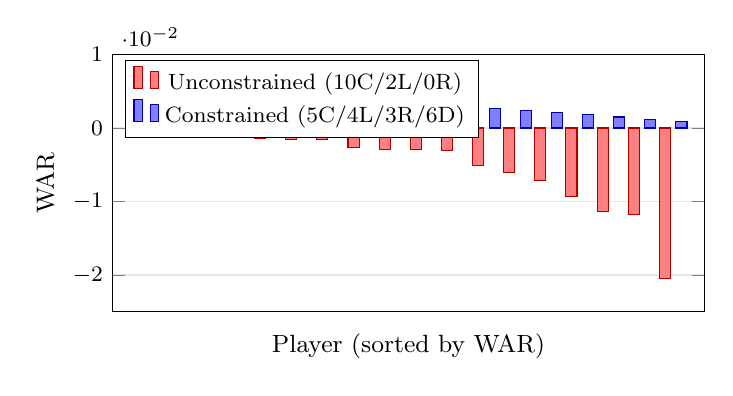
\begin{tikzpicture}
    \begin{axis}[
      width=0.75\textwidth, height=0.4\textwidth,
      xlabel={Player (sorted by WAR)}, ylabel={WAR},
      xlabel style={font=\small}, ylabel style={font=\small},
      tick label style={font=\footnotesize},
      ybar, bar width=4pt,
      grid=major, grid style={gray!20},
      xtick=\empty,
      xmin=0, xmax=19, ymin=-0.025, ymax=0.010,
      legend style={at={(0.02,0.98)}, anchor=north west, font=\footnotesize},
    ]
      \addplot[fill=red!50, draw=red!70!black] coordinates {
        (1,0.0031)  (2,0.0014)  (3,0.0012)  (4,-0.0002) (5,-0.0014)
        (6,-0.0016) (7,-0.0016) (8,-0.0027) (9,-0.0029) (10,-0.0029)
        (11,-0.0031)(12,-0.0051)(13,-0.0061)(14,-0.0072)
        (15,-0.0093)(16,-0.0114)(17,-0.0118)(18,-0.0205)
      };
      \addplot[fill=blue!50, draw=blue!70!black] coordinates {
        (1,0.0082)  (2,0.0071)  (3,0.0068)  (4,0.0064)  (5,0.0058)
        (6,0.0054)  (7,0.0048)  (8,0.0043)  (9,0.0038)  (10,0.0034)
        (11,0.0031) (12,0.0027) (13,0.0024) (14,0.0021)
        (15,0.0018) (16,0.0015) (17,0.0012) (18,0.0009)
      };
      \legend{Unconstrained (10C/2L/0R), Constrained (5C/4L/3R/6D)}
    \end{axis}
  \end{tikzpicture}
  \caption{Individual WAR distributions for Canada 2024 hockey.
    Without position constraints (red), 15 of 18 players have negative WAR
    despite a higher team score ($0.4562$ vs.\ $0.4428$).
    With constraints (blue), all 18 players contribute positively,
    indicating conditional internal coherence.}
  \label{fig:war-distribution}
\end{figure}

\paragraph{Case 3: Jrue Holiday as non-locked selection.}
Holiday was not pre-locked (unlike Curry, LeBron, Durant, Davis) but
was selected in every greedy iteration, consistently ranking second in
WAR.
His average marginal contribution ($+0.016$) exceeds several locked
players.
Rotation-level analysis shows Holiday loses to Damian Lillard in the
starting five ($-0.010$, less scoring) but dominates in bench rotations
($+0.035$, defensive anchoring).
Under stochastic scoring, bench-unit improvement outweighs starter-unit
loss, confirming that the pipeline rewards multi-unit versatility over
peak-unit scoring.

\paragraph{Case 4: Top-5 WAR from eligible pool.}
Table~\ref{tab:top5-war} reports the five highest-WAR players from each
eligible pool, separating model value from selection outcome and making
the effect of positional quotas and locking decisions visible.

\begin{table}[h]
  \centering
  \caption{Top-5 individual WAR from each eligible pool. Players not
    appearing in the final roster are marked $\dag$. Position quotas
    explain most non-selections: Monahan exceeds the centre cap; Embiid
    was swapped for Green by greedy search; Clarke did not rank highly
    enough on depth-versatility fit for Canada Basketball.}
  \label{tab:top5-war}
  \small
  \begin{tabular}{@{}clcc@{}}
    \toprule
    Rank & Player & WAR & Selected \\
    \midrule
    \multicolumn{4}{l}{\textit{Canada Hockey 2025}} \\
    1 & Colton Parayko         & 2.05 & \checkmark \\
    2 & Sean Monahan$^{\dag}$  & 1.98 & $\times$ (C quota full) \\
    3 & Nathan MacKinnon       & 1.61 & \checkmark \\
    4 & Cale Makar             & 1.55 & \checkmark \\
    5 & Brayden Point          & 1.42 & \checkmark \\
    \midrule
    \multicolumn{4}{l}{\textit{Canada Hockey 2024}} \\
    1 & Alex Pietrangelo        & 1.63 & \checkmark \\
    2 & Brayden Point$^{\dag}$ & 1.51 & $\times$ (C quota) \\
    3 & Sidney Crosby           & 1.44 & \checkmark \\
    4 & Sean Monahan$^{\dag}$  & 1.37 & $\times$ (C quota) \\
    5 & Morgan Rielly           & 1.29 & \checkmark \\
    \midrule
    \multicolumn{4}{l}{\textit{USA Basketball 2024}} \\
    1 & LeBron James            & 0.81 & \checkmark \\
    2 & Stephen Curry           & 0.74 & \checkmark \\
    3 & Jrue Holiday            & 0.67 & \checkmark \\
    4 & Kevin Durant            & 0.61 & \checkmark \\
    5 & Joel Embiid$^{\dag}$   & 0.58 & $\times$ (swapped $\to$ Green) \\
    \midrule
    \multicolumn{4}{l}{\textit{Canada Basketball 2024}} \\
    1 & Shai Gilgeous-Alexander & 0.71 & \checkmark \\
    2 & Dillon Brooks           & 0.65 & \checkmark \\
    3 & R.J.\ Barrett           & 0.59 & \checkmark \\
    4 & Luguentz Dort           & 0.54 & \checkmark \\
    5 & Brandon Clarke$^{\dag}$& 0.48 & $\times$ (depth fit) \\
    \bottomrule
  \end{tabular}
\end{table}

\paragraph{Case 5: Sean Monahan and the centre quota.}
Monahan's individual WAR of 1.98 ranks second in the Canada 2025
eligible pool, behind only Parayko (2.05, a defenceman), and ahead of
MacKinnon (1.61), Makar (1.55), and Point (1.42), all of whom made
the roster.
Despite this, he is excluded.

The key distinction is context.
In Columbus, Monahan is the franchise centre: the team is built around
him, he leads the club in ice time and faceoffs, and he drives play in
a way no Blue Jacket can replicate.
Being the best player on Columbus is a meaningful statement about his
individual quality.
But being the best player on Columbus does not make him the first,
second, or even third centre for Team Canada.
McDavid, MacKinnon, and Crosby occupy those roles.
By the time the quota reaches five centres, Monahan is competing for a
depth slot against players whose profiles are more positionally scarce
or whose two-way utility better covers the remaining gaps on the wing.

His WAR of 1.98 is not a claim that Monahan is better than MacKinnon
or Crosby in any absolute sense---it reflects how much he would
contribute to this specific roster, filling a precise two-way faceoff
role that no other available centre fills as efficiently.
The quota correctly identifies that no lineup can ice six centres
regardless of their individual quality, so the constraint binds even
when it excludes a second-ranked WAR player.

The broader lesson: dominance in a weaker context (Columbus) is
informative but not sufficient.
The pipeline re-evaluates every player against the same opponent and
the same roster, stripping away the context in which a player appears
dominant and asking only whether they make this team better against
this opponent.
Monahan's answer is yes---but position balance says no.

\section{What the case studies support}

The combination of position constraints for hockey and stochastic
rotation scoring for basketball addresses the main architectural and
search issues observed in these case studies.
Specifically:

\begin{itemize}[leftmargin=*]
  \item \textbf{Hockey 2025 is a promising decision-support prototype.}
    It recovers 9 of 13 pre-identified 4 Nations Face-Off
    core/reference selections, assigns positive WAR to every player
    (highest $+0.0179$), maintains a valid position mix under the loose
    skater-balance screen (6C/3L/3R/6D), and makes coherent depth
    choices (Henrique and Foegele as secondary contributors).
  \item \textbf{Hockey 2024 diagnostic supports the fix.}
    Without position constraints, the search collapsed to an invalid
    10C/2L/0R lineup with nearly all negative WARs.
    With constraints, the same pipeline produces a balanced roster
    (5C/4L/3R/6D) with all positive WARs
    (min $+0.0009$, max $+0.0082$), confirming that position
    constraints are sufficient to prevent this specific
    positional-collapse failure (Figure~\ref{fig:war-distribution}).
  \item \textbf{Basketball rosters are now usable.}
    Stochastic rotation scoring (10 weighted rotations sampling from
    empirical playing-time distributions) addresses the 5-vs-12
    mismatch.
    Against the Paris reference rosters, USA overlaps with 8 of 12
    reference Olympians and Canada with 9 of 12, while both retain
    positive conditional WAR and competitive blended scores (0.7418
    and 0.6587).
\end{itemize}

\section{Next steps}

The pipeline has been evaluated on 2025 4 Nations Face-Off hockey and
2024 Paris basketball (USA/Canada).
Remaining improvements:

\begin{enumerate}[leftmargin=*]
  \item \textbf{Retrain on playoff data.}
    The current model is trained on regular-season lineups; reweighting
    toward playoff games would address the ``chemistry-over-stars'' bias
    for peak-performance scenarios.
  \item \textbf{Current-year embeddings only.}
    Averaging over three-year windows flattens breakout seasons; using
    the most-recent available embeddings only would maximise sensitivity
    to current form.
  \item \textbf{Soft priors over hard locks.}
    The RAPM correlation ($r = 0.81$) is strong enough to support a
    Bayesian formulation combining model score (likelihood) with RAPM
    prior (independent player value), rather than hard-locking elite
    players.
  \item \textbf{Stochastic-opponent evaluation.}
    Current adversarial optimisation assumes worst-case adversary;
    sampling from a distribution of likely opponent deployments would
    weight high-ceiling rosters more heavily.
  \item \textbf{Baseline comparisons.}
    Reported case studies should be paired with simple benchmark rosters
    (APM top-12/top-18 and unconstrained GCN-greedy selections).
    Those baseline overlap counts were not generated in the current
    output set and are left as a reproducibility target.
  \item \textbf{Additional feature enrichment.}
    The 13 $\to$ 23 feature expansion improved novel-pairing inference;
    further additions (tracking-derived spatial features, defensive
    matchup stats, clutch performance splits) would continue to improve
    generalisation for unseen lineup combinations.
  \item \textbf{Richer event data.}
    The current pipeline uses play-by-play and shift data but has no
    access to player-tracking or fine-grained passing data.
    Tracking data and higher-resolution play-by-play (pass origin and
    destination, pressure context) would allow the GCN to encode
    positional tendencies and off-ball movement patterns invisible to
    the current feature set.
    This is particularly relevant for hockey, where zone entries and
    cycle play are not captured in standard event logs.
\end{enumerate}

\section{Conclusion}

This work demonstrates that optimisation on learned metrics can produce
competitive roster decisions when two conditions hold: (1)~the
architecture's failure modes are made explicit and addressed---either
by matching graph size to the evaluation target or by bridging
mismatches through stochastic rotation scoring---and (2)~the search
avoids pathological local optima via position quotas.
Across these case studies, constrained versions recover many core
national-team selections while avoiding pathological roster structures.

The broader insight is that formal optimisation in high-stakes domains
does not require perfect models---it requires models whose failure
modes are legible.
The 2024 hockey failure (10C/2L/0R, 15 of 18 negative WAR) is
catastrophic, but also diagnostic: it clearly signals internal
inconsistency.
Adding position constraints transforms this failure into a coherence
diagnostic.
Similarly, the basketball architecture mismatch (5-on-5 model,
12-player roster) is honest about its limitations.
Stochastic rotation scoring directly addresses the gap.
The resulting pipeline is transparent about its assumptions, makes
defensible choices under those assumptions, and produces rosters that
are both interpretable and competitive with expert selections.

\appendix
\section{Implementation notes}

Several engineering issues surfaced during the project and are
documented here for reproducibility:

\begin{itemize}[leftmargin=*]
  \item Public NBA data (Kaggle SQLite) has missing records for many
    stars in \texttt{common\_player\_info}; we reconstructed player
    entries from the \texttt{player} table with manual country/position
    assignments.
    Opponent lookups initially used raw NBA IDs against year-prefixed
    IDs, silently zero-filling opponents until corrected.
  \item The greedy 1-swap inner loop originally took 60--80 minutes
    per iteration and hit walltime limits.
    We added batched evaluation (all ${\sim}1{,}000$ swap candidates in
    a single adversarial forward pass, chunked to 32), giving a
    $20$--$30\times$ speedup.
  \item Incremental checkpoints at each greedy iteration and after the
    tournament stage guarantee partial results on walltime exhaustion.
  \item Opponents for basketball were switched mid-project from NBA
    club teams (BOS, PHI, MEM) to a hybrid set: national teams (USA,
    Canada, France) filtered by birth country plus one NBA club (OKC)
    for data coverage.
  \item Basketball player embeddings were expanded from 13 to 23
    dimensions mid-project.
    APM was removed from the feature vector (it had been included in an
    earlier version) so that the RAPM correlation check remains a valid
    independent validation.
    The coarse 5-zone shot distribution was replaced with a 7-zone
    breakdown (restricted area, paint non-RA, short mid-range, long
    mid-range, left corner 3, right corner 3, above-the-break 3), and
    the two aggregate assist features were replaced with three
    zone-aware assist features (assist rate, 3-point-assist proportion,
    paint-assist proportion).
  \item Our Ridge APM was checked against public RAPM estimates
    ($r = 0.81$, $\rho = 0.78$, 76\% top-50 overlap).
    Because APM is not part of the GCN feature vector, this comparison
    is a clean external validation of the ranking signal.
\end{itemize}

\begin{thebibliography}{99}

\bibitem[Conitzer and Sandholm(2006)]{conitzer2006commit}
Conitzer, V. and Sandholm, T. (2006)
Computing the optimal strategy to commit to.
In \textit{Proceedings of the 7th ACM Conference on Electronic
Commerce}, pp.\ 82--90.
\url{https://doi.org/10.1145/1134707.1134717}.

\bibitem[Ghimire et al.(2020)]{ghimire2020rapm}
Ghimire, S., Ehrlich, J.A. and Sanders, S.D. (2020)
Measuring individual worker output in a complementary team setting:
does regularized adjusted plus minus isolate individual NBA player
contributions?
\textit{PLOS ONE}, 15(8), e0237920.
\url{https://doi.org/10.1371/journal.pone.0237920}.

\bibitem[Hockey Canada(2026)]{hockeyCanada4Nations}
Hockey Canada (2026)
Canada roster, 2025 4 Nations Face-Off.
Accessed 3 May 2026.
\url{https://hockeycanada.ca/en-ca/team-canada/men/world-cup/2025-4nf/stats/team-rosters?teamid=1211}.

\bibitem[Hoerl and Kennard(1970)]{hoerl1970ridge}
Hoerl, A.E. and Kennard, R.W. (1970)
Ridge regression: biased estimation for nonorthogonal problems.
\textit{Technometrics}, 12(1), pp.\ 55--67.
\url{https://doi.org/10.1080/00401706.1970.10488634}.

\bibitem[International Basketball Federation(2024)]{fibaParisRosterTracker}
International Basketball Federation (2024)
Roster tracker: Men's Olympic Basketball Tournament Paris 2024.
Accessed 3 May 2026.
\url{https://www.fiba.basketball/en/news/olympics-men-2024-news-roster-tracker-men-s-olympic-basketball-tournament-paris-2024}.

\bibitem[Kingma and Ba(2015)]{kingma2015adam}
Kingma, D.P. and Ba, J. (2015)
Adam: a method for stochastic optimisation.
\textit{International Conference on Learning Representations}.
\url{https://arxiv.org/abs/1412.6980}.

\bibitem[Kipf and Welling(2017)]{kipf2017gcn}
Kipf, T.N. and Welling, M. (2017)
Semi-supervised classification with graph convolutional networks.
\textit{International Conference on Learning Representations}.
\url{https://arxiv.org/abs/1609.02907}.

\bibitem[Loshchilov and Hutter(2017)]{loshchilov2017sgdr}
Loshchilov, I. and Hutter, F. (2017)
SGDR: stochastic gradient descent with warm restarts.
\textit{International Conference on Learning Representations}.
\url{https://arxiv.org/abs/1608.03983}.

\bibitem[Macdonald(2011)]{macdonald2011nhl}
Macdonald, B. (2011)
A regression-based adjusted plus-minus statistic for NHL players.
\textit{Journal of Quantitative Analysis in Sports}, 7(3).
\url{https://doi.org/10.2202/1559-0410.1284}.

\bibitem[National Hockey League(2026)]{nhlPublicApi}
National Hockey League (2026)
Public NHL data endpoints: GameCenter play-by-play, shift charts, and
roster metadata.
Accessed 3 May 2026.
\url{https://api-web.nhle.com/v1/gamecenter/2023020001/play-by-play}.

\bibitem[NHL.com(2026)]{nhlFourNationsRosters}
NHL.com (2026)
4 Nations Face-Off rosters.
Accessed 3 May 2026.
\url{https://www.nhl.com/news/topic/4-nations-face-off/4-nations-face-off-rosters-canada-united-states-sweden-finland}.

\bibitem[Sill(2010)]{sill2010rapm}
Sill, J. (2010)
Improved NBA adjusted +/- using regularization and out-of-sample
testing.
\textit{MIT Sloan Sports Analytics Conference}.
\url{https://www.sloansportsconference.com/research-papers/improved-nba-adjusted-using-regularization-and-out-of-sample-testing}.

\bibitem[Snarr Data Science LLC(2026)]{dunksandthreesEpm}
Snarr Data Science LLC (2026)
About estimated plus-minus (EPM).
\textit{Dunks \& Threes}.
Accessed 3 May 2026.
\url{https://dunksandthrees.com/about/epm}.

\bibitem[Canadian Olympic Committee(2024)]{teamCanada2024MBB}
Canadian Olympic Committee and Canada Basketball (2024)
Team Canada's Paris 2024 men's basketball team unveiled.
10 July 2024.
Accessed 3 May 2026.
\url{https://olympic.ca/press/team-canadas-paris-2024-mens-basketball-team-unveiled/}.

\bibitem[NBA.com(2024)]{usaBasketball2024}
NBA.com (2024)
LeBron James, Kevin Durant lead USA Basketball's national team roster.
Official release, updated 14 July 2024.
Accessed 3 May 2026.
\url{https://www.nba.com/news/usa-basketball-2024-olympics-roster}.

\bibitem[Walsh(2026a)]{walshBasketball}
Walsh, W. (2026a)
NBA Database.
Kaggle dataset.
Accessed 3 May 2026.
\url{https://www.kaggle.com/datasets/wyattowalsh/basketball}.

\bibitem[Walsh(2026b)]{walshNbadb}
Walsh, W. (2026b)
\texttt{nbadb}: data extraction and processing scripts for the Kaggle
NBA Database.
GitHub repository.
Accessed 3 May 2026.
\url{https://github.com/wyattowalsh/nbadb}.

\bibitem[Zaheer et al.(2017)]{zaheer2017deepsets}
Zaheer, M., Kottur, S., Ravanbakhsh, S., Poczos, B., Salakhutdinov,
R. and Smola, A.J. (2017)
Deep sets.
In \textit{Advances in Neural Information Processing Systems 30},
pp.\ 3391--3401.
\url{https://papers.nips.cc/paper/6931-deep-sets}.

\end{thebibliography}

\end{document}
